\documentclass[10pt]{article}
%\usepackage{geometry}                % See geometry.pdf to learn the layout options. There are lots.
                 % ... or a4paper or a5paper or ... 
%\geometry{landscape}                % Activate for for rotated page geometry
%\usepackage[parfill]{parskip}    % Activate to begin paragraphs with an empty line rather than an indent
\usepackage[top=2cm, bottom=2cm, left=2cm, right=2cm]{geometry}
\geometry{letterpaper}  
\usepackage{graphicx}
\usepackage{amssymb}
\usepackage{amsmath}
\usepackage{epstopdf}
\usepackage{subfigure}
\usepackage[numbers]{natbib}
\DeclareGraphicsRule{.tif}{png}{.png}{`convert #1 `dirname #1`/`basename #1 .tif`.png}

%\title{Forgetting}
%\author{Frank Wood\\Columbia University\\Department of Statistics}
%\date{\today}                                           % Activate to display a given date or no date

% !TEX root = talk.tex

\newcommand{\comment}[1]{}
%\newcommand{\comment}[1]{{\marginpar{\tiny {#1} }}}
\def\todo#1{TODO(#1)}

\def\bigO{{\mathcal O}}
\def\balpha{\mbox{\boldmath $\alpha$}}
\def\bbeta{\mbox{\boldmath $\beta$}}
\def\beeta{\mbox{\boldmath $\eta$}}
\def\blambda{\mbox{\boldmath $\lambda$}}
\def\bmu{\mbox{\boldmath $\mu$}}
\def\bphi{\mbox{\boldmath $\phi$}}
\def\bpsi{\mbox{\boldmath $\psi$}}
\def\bsigma{\mbox{\boldmath $\sigma$}}
\def\btau{\mbox{\boldmath $\tau$}}
\def\btheta{\mbox{\boldmath $\theta$}}
\def\dbphi{\dot{\mbox{\boldmath $\phi$}}}
\def\dbtau{\dot{\mbox{\boldmath $\tau$}}}
\def\dbtheta{\dot{\mbox{\boldmath $\theta$}}}

%\newcommand{\nofootnotemark}{\let\@makefnmark\relax}
\newcommand{\bX}{\mathbf{X}}
\newcommand{\bY}{\mathbf{Y}}
\newcommand{\bW}{\mathbf{W}}
\newcommand{\bZ}{\mathbf{Z}}
\newcommand{\bH}{\mathbf{H}}
\newcommand{\bQ}{\mathbf{Q}}
\newcommand{\bA}{\mathbf{A}}
\newcommand{\bI}{\mathbf{I}}
\newcommand{\by}{\mathbf{y}}
\newcommand{\bz}{\mathbf{z}}
\newcommand{\bx}{\mathbf{x}}

\newcommand{\ith}{i^\mathrm{th}}
\def\A{{\bf A}}
\def\B{{\bf B}}
\def\C{{\bf C}}
\def\D{{\bf D}}
\def\F{{\bf F}}
\def\L{{\bf L}}
\def\M{{\bf M}}
\def\W{{\bf W}}
\def\I{{\bf I}}
\def\J{{\bf J}}
\def\R{{\bf R}}
\def\U{{\bf U}}
\def\V{{\bf V}}
\def\b{{\bf b}}
\def\c{{\bf c}}
\def\d{{\bf d}}
\def\r{{\bf r}}
\def\s{{\bf s}}
\def\t{{\bf t}}
\def\u{{\bf u}}
\def\v{{\bf v}}
\def\f{{\bf f}}
\def\x{{\bf x}}
\def\y{{\bf y}}
\def\w{{\bf w}}
\def\vo{{\bf o}}
\def\p{{\bf p}}
\def\O{{\bf 0}}
%\def\a{{\bf a}}


\def\vbpsi{\vec{\mbox{\boldmath $\psi$}}} 
\def\vpsi{\vec{\psi}} 
\def\vbphi{\vec{\mbox{\boldmath $\phi$}}} 
\def\vphi{\vec{\phi}} 
\def\vbtau{\vec{\mbox{\boldmath $\tau$}}} 
\def\vbtheta{\vec{\mbox{\boldmath $\theta$}}} 
\def\vD{\vec{D}}
\def\vf{\vec{\bf f}}
\def\vF{\vec{\bf F}}
\def\vI{\vec{\bf I}}
\def\vR{\vec{\bf R}}
\def\vv{\vec{v}}
\def\vV{\vec{\bf V}}

\def\pon{p_{\mathrm{on}}}
\def\poff{p_{\mathrm{off}}}

\def\tr{^{\text{T}}}

%%% Vector notation for sections 3 and 4
%%% Vector notation for sections 3 and 4
\def\mvec{\vec{m}}
\def\fvec{\vec{f}}
\def\appfvec{\vec{f}_k}
\def\avec{\vec{a}}
\def\bvec{\vec{b}}
\def\evec{\vec{e}}
\def\uvec{\vec{u}}
\def\xvec{\vec{x}}
\def\wvec{\vec{w}}
\def\gradvec{\vec{\nabla}}

\def\aM{\mbox{\bf a}_M}
\def\aS{\mbox{\bf a}_S}
\def\aO{\mbox{\bf a}_O}
\def\aL{\mbox{\bf a}_L}
\def\aP{\mbox{\bf a}_P}
\def\ai{\mbox{\bf a}_i}
\def\aj{\mbox{\bf a}_j}
\def\an{\mbox{\bf a}_n}
\def\a1{\mbox{\bf a}_1}
\def\a2{\mbox{\bf a}_2}
\def\a3{\mbox{\bf a}_3}
\def\a4{\mbox{\bf a}_4}

%\def\x{\mbox{\bf x\/}}
%\def\X{\mbox{\bf X}}
%\def\A{\mbox{\bf A}}
%\def\P{\mbox{\bf P}}
%\def\C{\mbox{\bf C}}
%\def\c{\mbox{\bf c}}
%\def\b{\mbox{\bf b}}
%\def\o{\mbox{\bf o}}
%\def\h{\mbox{\bf h}}
%\def\f{\mbox{\bf f}}
%\def\x{\mbox{\bf x}}
%\def\sx{\mbox{\scriptsize\bf x}}
%\def\z{\mbox{\bf z}}
%\def\l{\mbox{\bf l}}
%\def\m{\mbox{\bf m}}
%\def\bi{\mbox{\bf i}}
%\def\u{\mbox{\bf u}}
%\def\v{\mbox{\bf v}}
\def\a{\mbox{\bf a}}
%\def\p{\mbox{\bf p}}
%\def\r{\mbox{\bf r}}
%\def\d{\mbox{\bf d}}
%\def\Q{\mbox{\bf Q}}
%\def\s{\mbox{\bf s}}
%\def\st{\mbox{\scriptsize\bf t}}
%\def\ss{\mbox{\scriptsize\bf s}}
%\def\t{\mbox{\bf t}}
%\def\cR{{\cal R}}
%\def\calD{{\cal D}}
%\def\calS{{\cal S}}
%\def\g{\mbox{\bf g}}
%\def\e{\mbox{\bf e}}
%\def\flow{\{\mbox{\bf u}\}}
%\def\appearChange{iconic change}

\def\sigmae{\sigma}
\def\sigmam{\sigma}

\newcommand{\eg}{e.\thinspace{}g.,\@\xspace}
\newcommand{\egn}{e.\thinspace{}g.\@\xspace}
\newcommand{\cf}{cf.\@\xspace}
\newcommand{\ie}{i.\thinspace{}e.,\@\xspace}
\newcommand{\ien}{i.\thinspace{}e.\@\xspace}
\newcommand{\iid}{i.\thinspace{}i.\thinspace{}d.\@\xspace}


%\newcommand{\comment}[1]{}
\newcommand{\ponedec}{\mathcal{P}^\downarrow_1}
\newcommand{\pone}{\mathcal{P}_1}
\newcommand{\rank}[1]{\mathrm{RANK}\left[#1\right]}
\newcommand{\E}[1]{\mathrm{E}\left[#1\right]}
%\newcommand{\PY}{\mathcal{PY}}
%\newcommand{\DP}{\mathcal{DP}}
%\newcommand{\iid}{iid.}
\newcommand{\drawiid}{\stackrel{\text{iid}}{\sim}}
\newcommand{\vect}[1]{\mathbf{#1}}
\newcommand{\indicator}[1]{\text{I}\left[ #1 \right]}
\newcommand{\pdcoag}{PD(d_1,0)-\text{COAG}}
%\newcommand{\todo}{\textbf{*TODO*}}
\newcommand{\igram}{\text{$\infty$-gram}}
\newcommand{\Prob}{\text{P}}

\def\mm{sequence memoizer }
\def\MM{SM }

\def\pibf{{\boldsymbol{\pi}}}
\def\kapbf{\boldsymbol{\kappa}}
\def\taubf{\boldsymbol{\tau}}
\def\thebf{\boldsymbol{\theta}}
\def\rhobf{\boldsymbol{\rho}}
\def\phibf{\boldsymbol{\phi}}
\def\pbf{\mathbf{p}}
\def\qbf{\mathbf{q}}
\def\sbf{\mathbf{s}}
\def\tbf{\mathbf{t}}
\def\ybf{\mathbf{y}}
\def\ubf{\mathbf{u}}
\def\Ave{\mathbb{E}}

\def\wbf{\mathbf{w}}
\def\xbf{\mathbf{x}}
\def\rbf{\mathbf{r}}
\def\tbf{\mathbf{t}}
\def\kbf{\mathbf{k}}
\def\Xbf{\mathbf{X}}
\def\0bf{\mathbf{0}}
\def\Ibf{\mathbf{I}}
\def\phibf{\mathbf{\phi}}
\def\Phibf{\mathbf{\Phi}}
\def\disteq{{\stackrel{D}{=}}}
\def\EE{{\mathbb{E}}}
\def\GG{\mathcal{G}}
\def\G{G}
\def\U{U}

\def\phiv{\varphi}
\def\phivbf{\boldsymbol{\varphi}}

\def\Ocal{\mathcal{O}}
\DeclareMathOperator*{\Var}{Var}

\DeclareMathOperator*{\Bet}{Beta}
\DeclareMathOperator{\coag}{COAG}
\DeclareMathOperator{\frag}{FRAG}
\DeclareMathOperator*{\rnk}{RANK}
\DeclareMathOperator*{\gem}{GEM}
\DeclareMathOperator*{\pd}{PD}
\DeclareMathOperator*{\py}{PY}
\DeclareMathOperator*{\DP}{DP}
\DeclareMathOperator*{\PY}{PY}
\DeclareMathOperator*{\gd}{GDir}
\DeclareMathOperator*{\Dir}{Dir}
\DeclareMathOperator*{\CRP}{CRP}
\DeclareMathOperator*{\argmax}{argmax}



%%% Local Variables: 
%%% mode: latex
%%% TeX-master: "paper"
%%% End: 
% !TEX root = talk.tex
%
%\newcommand{\comment}[1]{}
%%\newcommand{\comment}[1]{{\marginpar{\tiny {#1} }}}
%
%\def\bigO{{\mathcal O}}
%\def\balpha{\mbox{\boldmath $\alpha$}}
%\def\bbeta{\mbox{\boldmath $\beta$}}
%\def\beeta{\mbox{\boldmath $\eta$}}
%\def\blambda{\mbox{\boldmath $\lambda$}}
%\def\bmu{\mbox{\boldmath $\mu$}}
%\def\bphi{\mbox{\boldmath $\phi$}}
%\def\bpsi{\mbox{\boldmath $\psi$}}
%\def\bsigma{\mbox{\boldmath $\sigma$}}
%\def\btau{\mbox{\boldmath $\tau$}}
%\def\btheta{\mbox{\boldmath $\theta$}}
%\def\dbphi{\dot{\mbox{\boldmath $\phi$}}}
%\def\dbtau{\dot{\mbox{\boldmath $\tau$}}}
%\def\dbtheta{\dot{\mbox{\boldmath $\theta$}}}
%
%%\newcommand{\nofootnotemark}{\let\@makefnmark\relax}
%\newcommand{\bX}{\mathbf{X}}
%\newcommand{\bY}{\mathbf{Y}}
%\newcommand{\bW}{\mathbf{W}}
%\newcommand{\bZ}{\mathbf{Z}}
%\newcommand{\bH}{\mathbf{H}}
%\newcommand{\bQ}{\mathbf{Q}}
%\newcommand{\bA}{\mathbf{A}}
%\newcommand{\bI}{\mathbf{I}}
%\newcommand{\by}{\mathbf{y}}
%\newcommand{\bz}{\mathbf{z}}
%\newcommand{\bx}{\mathbf{x}}
%
%\newcommand{\ith}{i^\mathrm{th}}
%\def\A{{\bf A}}
%\def\B{{\bf B}}
%\def\C{{\bf C}}
%\def\D{{\bf D}}
%\def\F{{\bf F}}
%\def\L{{\bf L}}
%\def\M{{\bf M}}
%\def\W{{\bf W}}
%\def\I{{\bf I}}
%\def\J{{\bf J}}
%\def\R{{\bf R}}
%\def\U{{\bf U}}
%\def\V{{\bf V}}
%\def\b{{\bf b}}
%\def\c{{\bf c}}
%\def\d{{\bf d}}
%\def\r{{\bf r}}
%\def\s{{\bf s}}
%\def\t{{\bf t}}
%\def\u{{\bf u}}
%\def\v{{\bf v}}
%\def\f{{\bf f}}
%\def\x{{\bf x}}
%\def\y{{\bf y}}
%\def\w{{\bf w}}
%\def\vo{{\bf o}}
%\def\p{{\bf p}}
%\def\O{{\bf 0}}
%%\def\a{{\bf a}}
%
%
%\def\vbpsi{\vec{\mbox{\boldmath $\psi$}}} 
%\def\vpsi{\vec{\psi}} 
%\def\vbphi{\vec{\mbox{\boldmath $\phi$}}} 
%\def\vphi{\vec{\phi}} 
%\def\vbtau{\vec{\mbox{\boldmath $\tau$}}} 
%\def\vbtheta{\vec{\mbox{\boldmath $\theta$}}} 
%\def\vD{\vec{D}}
%\def\vf{\vec{\bf f}}
%\def\vF{\vec{\bf F}}
%\def\vI{\vec{\bf I}}
%\def\vR{\vec{\bf R}}
%\def\vv{\vec{v}}
%\def\vV{\vec{\bf V}}
%
%\def\pon{p_{\mathrm{on}}}
%\def\poff{p_{\mathrm{off}}}
%
%\def\tr{^{\text{T}}}
%
%%%% Vector notation for sections 3 and 4
%%%% Vector notation for sections 3 and 4
%\def\mvec{\vec{m}}
%\def\fvec{\vec{f}}
%\def\appfvec{\vec{f}_k}
%\def\avec{\vec{a}}
%\def\bvec{\vec{b}}
%\def\evec{\vec{e}}
%\def\uvec{\vec{u}}
%\def\xvec{\vec{x}}
%\def\wvec{\vec{w}}
%\def\gradvec{\vec{\nabla}}
%
%\def\aM{\mbox{\bf a}_M}
%\def\aS{\mbox{\bf a}_S}
%\def\aO{\mbox{\bf a}_O}
%\def\aL{\mbox{\bf a}_L}
%\def\aP{\mbox{\bf a}_P}
%\def\ai{\mbox{\bf a}_i}
%\def\aj{\mbox{\bf a}_j}
%\def\an{\mbox{\bf a}_n}
%\def\a1{\mbox{\bf a}_1}
%\def\a2{\mbox{\bf a}_2}
%\def\a3{\mbox{\bf a}_3}
%\def\a4{\mbox{\bf a}_4}
%
%%\def\x{\mbox{\bf x\/}}
%%\def\X{\mbox{\bf X}}
%%\def\A{\mbox{\bf A}}
%%\def\P{\mbox{\bf P}}
%%\def\C{\mbox{\bf C}}
%%\def\c{\mbox{\bf c}}
%%\def\b{\mbox{\bf b}}
%%\def\o{\mbox{\bf o}}
%%\def\h{\mbox{\bf h}}
%%\def\f{\mbox{\bf f}}
%%\def\x{\mbox{\bf x}}
%%\def\sx{\mbox{\scriptsize\bf x}}
%%\def\z{\mbox{\bf z}}
%%\def\l{\mbox{\bf l}}
%%\def\m{\mbox{\bf m}}
%%\def\bi{\mbox{\bf i}}
%%\def\u{\mbox{\bf u}}
%%\def\v{\mbox{\bf v}}
%\def\a{\mbox{\bf a}}
%%\def\p{\mbox{\bf p}}
%%\def\r{\mbox{\bf r}}
%%\def\d{\mbox{\bf d}}
%%\def\Q{\mbox{\bf Q}}
%%\def\s{\mbox{\bf s}}
%%\def\st{\mbox{\scriptsize\bf t}}
%%\def\ss{\mbox{\scriptsize\bf s}}
%%\def\t{\mbox{\bf t}}
%%\def\cR{{\cal R}}
%%\def\calD{{\cal D}}
%%\def\calS{{\cal S}}
%%\def\g{\mbox{\bf g}}
%%\def\e{\mbox{\bf e}}
%%\def\flow{\{\mbox{\bf u}\}}
%%\def\appearChange{iconic change}
%
%\def\sigmae{\sigma}
%\def\sigmam{\sigma}
%
%\newcommand{\eg}{e.\thinspace{}g.,\@\xspace}
%\newcommand{\egn}{e.\thinspace{}g.\@\xspace}
%\newcommand{\cf}{cf.\@\xspace}
%\newcommand{\ie}{i.\thinspace{}e.,\@\xspace}
%\newcommand{\ien}{i.\thinspace{}e.\@\xspace}
%\newcommand{\iid}{i.\thinspace{}i.\thinspace{}d.\@\xspace}
%
%
%%\newcommand{\comment}[1]{}
%\newcommand{\ponedec}{\mathcal{P}^\downarrow_1}
%\newcommand{\pone}{\mathcal{P}_1}
%\newcommand{\rank}[1]{\mathrm{RANK}\left[#1\right]}
%%\newcommand{\E}[1]{\mathrm{E}\left[#1\right]}
%%\newcommand{\PY}{\mathcal{PY}}
%%\newcommand{\DP}{\mathcal{DP}}
%%\newcommand{\iid}{iid.}
%\newcommand{\drawiid}{\stackrel{\text{iid}}{\sim}}
%\newcommand{\vect}[1]{\mathbf{#1}}
%\newcommand{\indicator}[1]{\text{I}\left[ #1 \right]}
%\newcommand{\pdcoag}{PD(d_1,0)-\text{COAG}}
%%\newcommand{\todo}{\textbf{*TODO*}}
%\newcommand{\igram}{\text{$\infty$-gram}}
%\newcommand{\Prob}{\text{P}}
%
%\def\mm{sequence memoizer }
%\def\MM{SM }
%
%\def\pibf{{\boldsymbol{\pi}}}
%\def\kapbf{\boldsymbol{\kappa}}
%\def\taubf{\boldsymbol{\tau}}
%\def\thebf{\boldsymbol{\theta}}
%\def\rhobf{\boldsymbol{\rho}}
%\def\phibf{\boldsymbol{\phi}}
%\def\pbf{\mathbf{p}}
%\def\qbf{\mathbf{q}}
%\def\sbf{\mathbf{s}}
%\def\tbf{\mathbf{t}}
%\def\ybf{\mathbf{y}}
%\def\ubf{\mathbf{u}}
%\def\Ave{\mathbb{E}}
%
%\def\wbf{\mathbf{w}}
%\def\xbf{\mathbf{x}}
%\def\rbf{\mathbf{r}}
%\def\tbf{\mathbf{t}}
%\def\kbf{\mathbf{k}}
%\def\Xbf{\mathbf{X}}
%\def\0bf{\mathbf{0}}
%\def\Ibf{\mathbf{I}}
%\def\phibf{\mathbf{\phi}}
%\def\Phibf{\mathbf{\Phi}}
%\def\disteq{{\stackrel{D}{=}}}
%\def\GG{\mathcal{G}}
%\def\G{G}
%\def\U{U}
%
%\def\phiv{\varphi}
%\def\phivbf{\boldsymbol{\varphi}}
%
%\def\Ocal{\mathcal{O}}
%\DeclareMathOperator*{\Var}{Var}
%
%\DeclareMathOperator*{\Bet}{Beta}
%\DeclareMathOperator{\coag}{COAG}
%\DeclareMathOperator{\frag}{FRAG}
%\DeclareMathOperator*{\rnk}{RANK}
%\DeclareMathOperator*{\gem}{GEM}
%\DeclareMathOperator*{\pd}{PD}
%\DeclareMathOperator*{\py}{PY}
%\DeclareMathOperator*{\DP}{DP}
%\DeclareMathOperator*{\PY}{PY}
%\DeclareMathOperator*{\gd}{GDir}
%\DeclareMathOperator*{\Dir}{Dir}
%\DeclareMathOperator*{\CRP}{CRP}
%\DeclareMathOperator*{\argmax}{argmax}
%
\def\GG{\mathcal{G}}
\def\data{\mathbf{x}}
%\def\EE{\mathbb{E}}
\def\disc{d}
%\newcommand{\delete}[1]{} %\textcolor{red}{#1}
%\newcommand{\rewrite}[1]{#1}%{\textcolor{blue}{#1}} %
%\newcommand{\lambdabf}{\boldsymbol{\lambda}}
%\newcommand{\vbf}{\mathbf{v}}
%\newcommand{\Psmooth}{\Prob_\text{smooth}}
%%\newcommand{\parent}{\pi}
%\newcommand{\suffix}{\sigma}
%\newcommand{\UHPYP}{SM}
%\newcommand{\PLUMP}{PLUMP}
%\newcommand{\Oh}{\mathcal{O}}
%\newcommand{\tree}{\mathcal{T}}
\newcommand{\cct}{\hat{\mathcal{T}}}
\newcommand{\cctx}{\cct(\data)}
\newcommand{\Gu}{G_{\ubf}}
%\newcommand{\GuSet}{\{G_{\ubf}\}_{\ubf \in \Sigma^*}}
%\newcommand{\E}{\mathrm{E}}
%\newcommand{\UpdatePath}{\text{\textsc{UpdatePath}}}
%\newcommand{\Path}{\ensuremath{(\ubf_0,\ldots,\ubf_P)}}
%\newcommand{\PathProbability}{\text{\textsc{PathProbability}}}
%\newcommand{\TT}{\mathcal{T}}
%\newcommand{\ral}[1]{\stackrel{\mathtt{#1}}{\rightarrow}}
\def\parent{{\sigma(\mathbf{u})}}
%
%%\def\newblock{\hskip .11em plus .33em minus .07em}
%
%
%% \newcommand{\cusk}{c_{\ubf s k}}
%% \newcommand{\cus}{c_{\ubf s \cdot}}
%% \newcommand{\cu}{c_{\ubf \cdot \cdot}}
%% \newcommand{\tus}{t_{\ubf s}}
%% \newcommand{\tu}{t_{\ubf \cdot}}
%\newcommand{\cusk}{c_{\ubf s k}}
%\newcommand{\cus}{c_{\ubf s}}
%\newcommand{\cu}{c_{\ubf \cdot}}
%\newcommand{\tus}{t_{\ubf s}}
%\newcommand{\tu}{t_{\ubf \cdot}}
%\newcommand{\cset}{\{\cusk\}_{s\in \Sigma,k \in \{1,\ldots,t_{\ubf s}\}}}
%\newcommand{\tset}{\{\tus\}_{s\in \Sigma}}
%\newcommand{\bydef}{\equiv}
%\newcommand{\state}{\mathcal{S}_{\xbf}}
%\newcommand{\statei}{\mathcal{S}_{\xbf_{1:i}}}
%%\newcommand{\emptystring}{\varepsilon}
%\newcommand{\gcount}{\hat{c}}
%\newcommand{\escape}{\mathtt{esc}}
%\def\prob{G}
%
%
%\newcommand{\todo}[1]{\begin{center}\textbf{TODO: } #1 \end{center}}
%\newcommand{\figref}[1]{\figurename~\ref{#1}}
%\newcommand{\predictive}{\Prob(x_i|\xbf_{1:i-1})}
%\newcommand{\ywcomment}[1]{\textbf{#1}}
%\newcommand{\jgcomment}[1]{ { \textcolor{red}{#1} } }
%
%\newcommand{\secref}[1]{Section \ref{#1}}
%
\def\context{\mathbf{u}}

%%% Local Variables: 
%%% mode: latex
%%% TeX-master: "paper"
%%% End: 


\begin{document}
%\maketitle
\begin{center} \bf \Large Scalable sequence memoization for natural language modeling and lossless compression.\end{center}
%
%A Step Towards Fully-Unsupervised, Life-Long, Incremental Learning

%Exploring the marriage of massive data to unsupervised, deep hierarchical nonparametric Bayesian learners.
%\section{Principle Investigators}
%
\begin{center}
\begin{tabular}{llll}
{\bf PI }& Frank Wood, Ph.D. &{\bf Position }& Assistant Professor\\
{\bf Co-PI}& David Madigan, Ph.D. &{\bf Position  }& Professor\\
{\bf Address} & Room 1005 SSW, MC 4690 & {\bf University} & Columbia University \\
&1255 Amsterdam Avenue & {\bf Department }& Statistics \\
&New York, NY 10027 \\
 {\bf Phone} & 212.851.2132& {\bf Fax} & 212.851.2164 \\
 {\bf Websites} &{http://www.stat.columbia.edu/$\sim$fwood}\\
 & \multicolumn{2}{l}{http://www.stat.columbia.edu/$\sim$madigan}
\end{tabular}
\end{center}

%\subsection{Abstract}
\begin{quote}
\begin{center}
\bf Abstract
\end{center}
 We propose to develop and demonstrate scalable inference software for a Bayesian nonparametric (BNP) natural language model called the sequence memoizer (SM) \citep{Wood2009}.  We propose to use this software to train a SM using the trillion word Google text corpus and to empirically study the effect of taking into account long-range textual dependencies on language model performance as the amount of training data grows.   We also propose to develop a latent variable extension of the SM and demonstrate scalable inference in the same.  We propose to demonstrate
both models and algorithms in two ways, general purpose lossless
compression and $n$-gram natural language model performance.

%\vspace{-.05cm}
{\bf Keywords :} Bayesian nonparametric inference,  $n$-gram natural language modeling, sequence memoizer

\vspace{-.1cm}
{\bf Research Areas :} language modeling, machine translation, automated speech recognition, compression
\end{quote}
%\subsection{Goals}

\noindent {\bf Goals } 
\begin{itemize}
\item Develop a freely available, downloadable software development kit (SDK) that contains a scalable implementation of a constant space, linear time SM language model that demonstrably scales to sequences that are billions to trillions of tokens long.
\item Empirically explore the impact of being able to probabilistically model and exploit long contextual dependencies given Google-scale corpora on language model perplexity and compressor log-loss.
%\item Define an extension to the sequence memoizer by combining it with a latent variable process.%for instance, the infinite hierarchical Markov model \citep{Heller2009} or latent Dirichlet allocation \citep{Blei2003}.
%\item Develop scalable incremental estimation procedures for the combined model.
\end{itemize}

\noindent {\bf Expected Outcomes } 
\begin{itemize}
\item The primary result of this project will be the establishment of compelling evidence that supports the practicality and usefulness of Bayesian nonparametric language models for large scale commercial applications including machine translation, automated speech detection, and general purpose lossless compression.
\item We will develop a SM SDK that will be downloaded and used by researchers in a wide-variety of industrial and academic fields.
\item We will contribute to the state of the art in Bayesian nonparametric modeling by developing an latent variable extension to the SM.
%\item We anticipate improving on the language model and compression performance of the sequence memoizer by extending the model to include a latent variable process.
%\item Define an extension to the sequence memoizer by combining it with a latent variable process.%for instance, the infinite hierarchical Markov model \citep{Heller2009} or latent Dirichlet allocation \citep{Blei2003}.
%\item Develop scalable incremental estimation procedures for the combined model.
\end{itemize}

\noindent{\bf \large Big Picture}
\vspace{.2cm}

Traditional parametric statistical tools and methods are designed to allow
inference about a population from a small sample.
While this parametric style of inference will always have a place, it is now the
case that one often has access to so much data that parametric models
themselves are sometimes not even necessary.  In other words, for some problems one can do strict nonparametric inference; i.e.~one can query
the data directly.  While such a nonparametric approach has attractive characteristics and  for some problems is feasible to consider, particularly given Google-scale data, we suggest that there are stochastic processes of sufficient complexity (e.g.~natural language generators) that strictly nonparametric approaches to estimation and inference (e.g.~non-smoothed $n$-gram language models) are bound to fail.  To attack these kinds of problems, we advocate and actively pursue computationally practical ways to estimate and perform inference in Bayesian nonparametric (BNP) models.   BNP models are nonparametric in nature, which gives them inferential capacity that can be understood to grow as a function of the amount of training data. Contrast this to parametric models in which inference is limited to inference through and about a finite set of parameters.   In parametric models as the amount of data grows, posterior uncertainty about the value of the parameters will vanish given sufficient data, rendering the inclusion of additional data irrelevant.  This is not true for BNP models, making them ideal for inference in the modern regime of continually growing data.  BNP models are are also Bayesian in nature which allows for hierarchical Bayesian-style regularization and incremental Bayesian-style inference and estimation.  For small scale data on the order of millions of observations, BNP natural language models and lossless compressors we have recently been shown to exhibit excellent empirical characteristics \citep{Teh2006a,Wood2009,Gasthaus2010}.  Unfortunately BNP models in general have been saddled with an unfortunate stigma, namely that they are as a class uniformly computationally complex. We suspect that this stigma is at least partially responsible for holding back wide adoption of BNP methods.   The work outlined in this proposal aims to chip away at this stigma by providing concrete evidence that at least one member of this class of BNP models scales well.

\vspace{.2cm}
\noindent{\bf \large Scaling the Sequence Memoizer}
\vspace{.2cm}

In recent work we established a rather surprising result: for non-antagonistically generated discrete sequence data (natural language token sequences, bytes, bits, etc.), we found that it was possible to estimate  the SM in the same asymptotic space and time as is required to estimate a smoothing $5$-gram model \citep{Wood2009} (\figref{fig1a}).  One way to understand the SM is as a Bayesian smoothing $n$-gram model in the limit of $n$ taken to infinity.  This means that the SM is capable of modeling long-range dependencies in discrete sequence data as opposed to finite-order Markov models which cannot.  What is more, in related work, we uncovered empirical evidence that supports Shannon's assertion \citep{Shannon1951} that long range dependencies in written language do exist and are significant up to and potentially extend beyond hundreds of characters \cite{Gasthaus2010} (related evidence for this can also be seen in \figref{fig1b}).  
\begin{figure}[htbp]
\begin{center}
\subfigure[]{
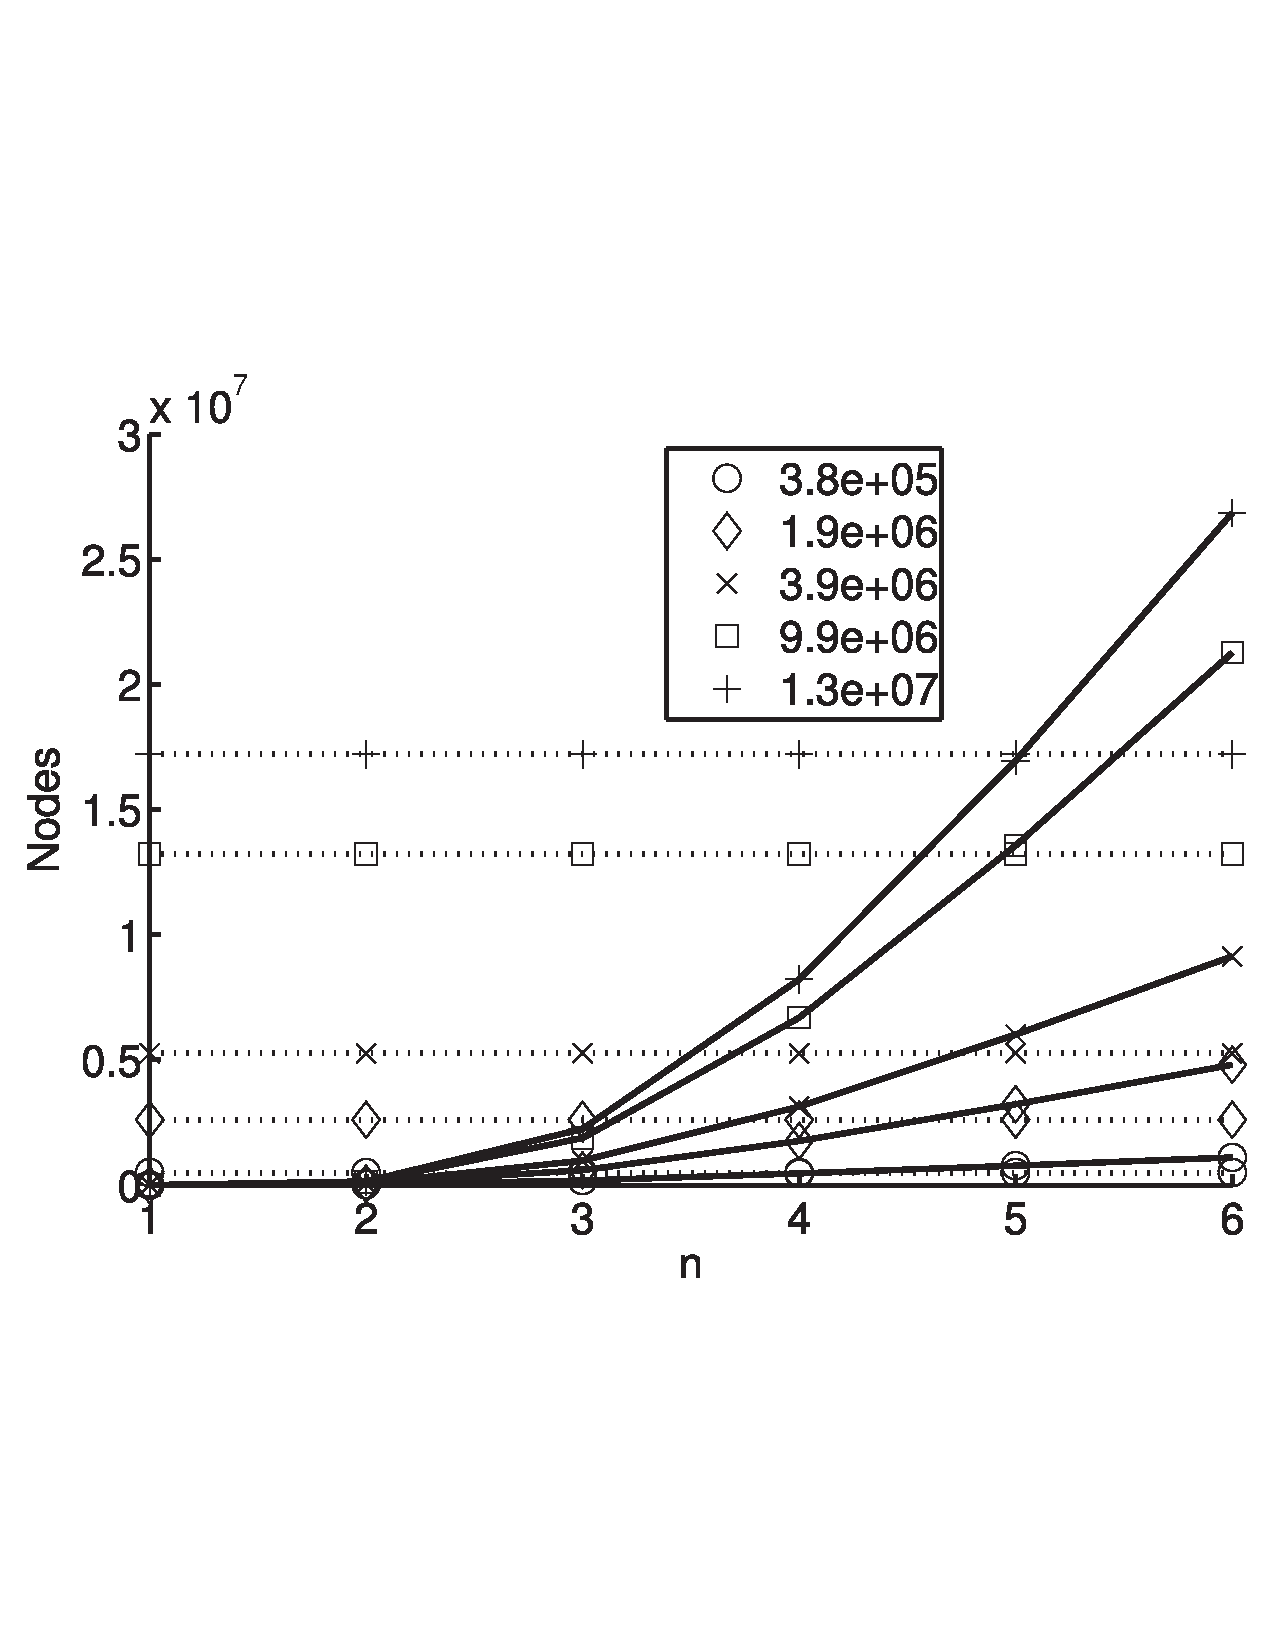
\includegraphics[trim = 0mm 60mm 00mm 60mm, clip, width=.4\textwidth]{fig1b.pdf}
\label{fig1a}
}
\hspace{1.5cm}
\subfigure[]{
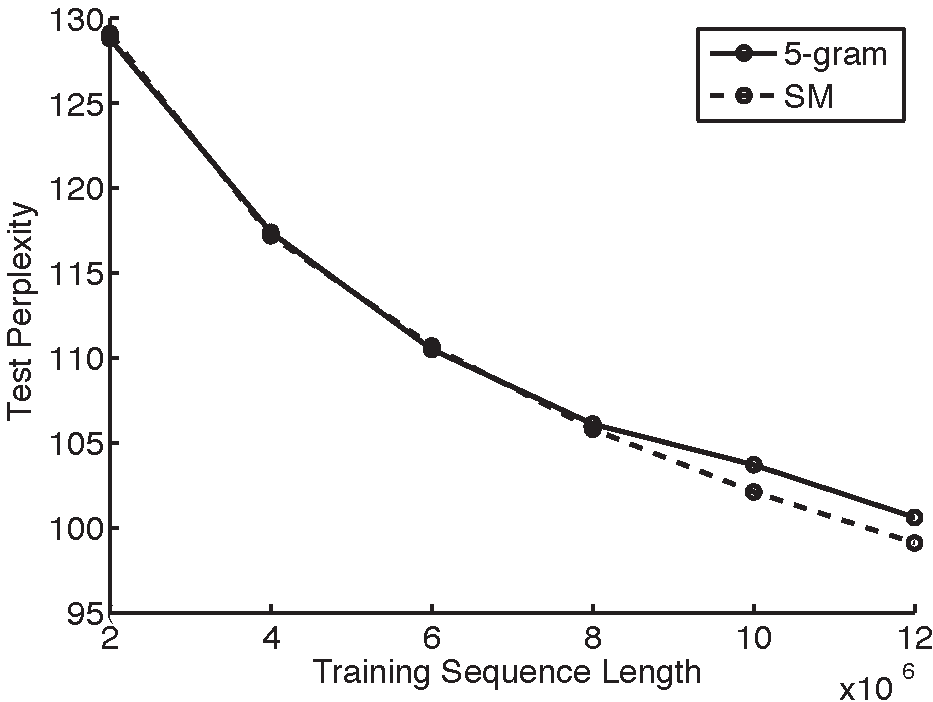
\includegraphics[width=.4\textwidth]{fig1.pdf}
\label{fig1b}
}
\caption{(a)  Memory complexity and estimation computational cost (in units of graphical model ``nodes'') versus $n$ of $n$-gram for the SM and a smoothing $n$-gram model.  There is one pair of lines for each of 5 different observation sequence lengths.  The horizontal dotted lines are the SM computational requirements.  The quadratic solid lines are the computational requirements the  smoothing $n$-gram models.  The SM always uses all contextual information when performing predictive inference.  The $n$-gram model discards contextual observations more distant than $n-1$.  None-the-less (a) shows that the computational complexity of each standard $n$-gram model exceeds that of a sequence memoizer trained on the same data for all $n>5$ and for all training observation sequence lengths.  This suggests that the sequence memoizer should be considered as an alternative to $n$-gram language modeling if long-range contextual dependencies matter.  The data used in this experiment was an excerpt of the New York times corpus.  (b)  Held-out test perplexity for two language models trained on growing excerpts of the Associated Press news corpus.  5-gram is a hierarchical Pitman-Yor process language model (a generalization of a Kneser Ney smoothed 5-gram model).  SM is the sequence memoizer.  Training sequence length ranges from 2-12 million tokens which we believe to be too small to characterize the benefit of being able to model and use long range dependencies.  Regardless, (b) suggests that held-out perplexity under the SM seems to improve relative to the smoothed $n$-gram model as more data is introduced into the model.  We conjecture that this is due to increasing prevalence of meaningful long contexts.  Experiments such as those proposed herein on larger corpora would establish the veracity of this conjecture.  Both of these figures were taken from \cite{Wood2009}.}
\label{default}
\end{center}
\end{figure}

We have already begun to demonstrate the practical utility of the SM, and in particular the benefits it extends beyond fixed, finite-depth $n$-gram models.  Various studies have found evidence of improvements to natural language models for automated speech recognition and machine translation, better encoding models for lossless compressors, and so forth.  These benefits seem to accrue from by being able to model and use the extra information that longer contexts provide, but much more experimentation is required to verify this observation.  We feel that an important scientific question remains unanswered: what happens to the importance of long-range contextual information as the amount of training data is increased?  Our intuition suggests that long-range dependencies will become more valuable, and the advantage of the SM relative to $n$-gram language models will grow, but currently the answer to this question remains unknown.   Further, the software and hardware infrastructure needed to answer this question do not currently exist.  One of the main purposes of this proposal is to start to address this question.

We have taken several theoretical and practical steps beyond the initial version of the SM; incremental estimation of the SM and the coupling of it to an entropy coder resulted in a highly competitive general purpose lossless compressor (significantly better than, for instance, gzip and bzip2) that scaled sufficiently to encode and compress a 100MB wikipedia corpus (1.6 bits / byte) \citep{Gasthaus2010}.  Following on that work, we have taken steps towards the development of a constant space, linear time approach to estimation of a class of models that includes the SM  \citep{Bartlett2010}.  This work  opens up for the first the possibility of performing experiments on large scale sequence data including the tera-word Google corpus.   No one knows what will happen when a powerful NPB language model such as the SM is trained on orders of magnitude more data than ever before.  Most of the engineering work necessary to achieve the asymptotic complexity results established in \citep{Bartlett2010} (constant space storage, linear time estimation, constant time inference) remains to be done, but we know it can be.  This means that many of the most interesting questions about the value of long-range contextual dependencies and the inferential power of BNP language models finally have a chance to be answered.

%In the course of pursuing this line of research, several pressing questions have emerged, the answers to which both have significant practical and theoretical importance.  We propose to answer these questions over the course of this project.

\comment{
\vspace{.2cm}
\noindent{\bf \large Sequence Memoizer}
\vspace{.2cm}

The SM \citep{Wood2009} consists of a hierarchical Bayesian nonparametric \citep{Teh2006a} prior
composed of Pitman-Yor processes married to efficient methods for representing and doing Bayesian inference in the resulting model. 
\def\GG{\mathcal{G}} The sequence memoizer describes the conditional probability of each
symbol $s$ following each context $\ubf$ using a latent variable $G_\ubf(s).$  Each symbol $s$ is a member of a set of symbols $\Sigma$.  
Collecting the natural set of such variables into a vector, $G_\ubf=[G_\ubf(s)]_{s\in\Sigma}$ results in $G_\ubf$ being a
probability vector (non-negative entries summing to one).   There is one such distribution for every context $\ubf$.    The full
(infinite) set of latent variables in the model (all the nodes in an infinitely deep tree) is denoted by
$\GG=\{G_\ubf\}_{\ubf\in\Sigma^*}$.  




The joint\footnote{Recall that a joint distribution can always be factored into the product of conditional distributions of increasing context, i.e.~$P(x_1,\ldots,x_i|\theta) = P(x_1|\theta) P(x_2 | x_1, \theta) P(x_3 | x_1,x_2, \theta) \cdots P(x_i | \xbf_{1:(i-1)}, \theta)$} probability of $\xbf$ and $\GG$
is simply:
\begin{align}
P(\xbf,\GG) = P(\GG)\prod_{i=0}^{|\xbf|-1}G_{\xbf_{1:i}}(\xbf_{i+1})
\end{align}
where the rightmost term is the probability of each symbol conditioned on the sequence thus far, and $P(\GG)$ is the prior over the variables.  Bayesian inference is possible in this model and means that one can integrate out $\GG$ (by sequential importance sampling and Monte Carlo integration for instance), to get a marginal joint distribution $P(\xbf)$ over the sequence from which the various predictive distributions of interest can straightforwardly be derived.  
%Section \ref{sec:inference} describes how the algorithm in Section \ref{algorithm} is an approximation of this ideal Bayesian approach.

The prior used in the SM over the infinite set $\GG=\{G_\ubf\}_{\ubf\in\Sigma^*}$ of probability vectors is based on a hierarchical Bayesian model consisting of Pitman Yor processes.
\comment{\footnote{
In this paper we exclusively refer to a simplified Pitman-Yor process.  The Pitman-Yor process (PYP) \citep{Pitman1997}, denoted $\py(d,H)$, is a
distribution over probability vectors.   
It is parameterized by a \emph{discount parameter} $d \in (0,1)$ and a
probability vector $H$ called the \emph{base vector}.  If $G\sim\py(d,H)$ is a
Pitman-Yor distributed random probability vector, then the base vector is
simply its mean $\text{E}[G(s)]=H(s)$ while the discount parameter is related
to its variance $\text{Var}[G(s)]=(1-d)H(s)(1-H(s))$, for each $s\in\Sigma$.}}
%
%The sequence memoizer \citep{wood2009sms} is an extension of the general HPYP
%model described above to context of unbounded length, i.e. $\ubf$ is not
%restricted to maximum length, leading to a context tree of unbounded depth. 
%In order to make inference in such a model feasible through marginalization
%(described in the next paragraph), the parameter space of
%the PYP has to be restricted to $\alpha=0$. 
Succinctly, we can notate the SM prior as follows:
\begin{subequations}
        \label{eqn:sm_prior}
        \begin{align}
            G_{\varepsilon} \mid d_0,H\quad &\sim \quad\py(d_0,H) \label{eq:m1} &\\
            G_{\ubf} \mid d_{|\ubf|},G_{\suffix(\ubf)} \quad
            &\sim \quad \py(d_{|\ubf|},G_{\suffix(\ubf)})  & \forall \ubf \in
            \Sigma^+ \label{eq:m2}\\
            x_i \mid \xbf_{1:i-1}=\ubf \quad &\sim\quad  G_{[\ubf]} 
            &  
            i=1,\ldots,T \label{eq:m3}
        \end{align}
\end{subequations}
\noindent where $H$ is a base probability distribution vector (in the following assumed to be
uniform over a finite vocabulary) and $d_{|\ubf|}$ are PYP parameters.
%The SM model is a hierarchical prior placed on the set of distributions
%$\{G_{[\ubf]}\}_{\ubf \in \Sigma^{*}}$, where $G_{[\ubf]}(v)$  corresponds
%to the probability of symbol $v \in \Sigma$ following the context $\ubf$.
%The structure of the model is an unbounded-depth tree, with each node indexed by a context $\ubf\in\Sigma^*$, labelled by the probability vector $G_\ubf$, and with parent given by $\sigma(\ubf)$.   %A binary sequence memoizer model is shown in Fig.~\ref{fig: gm_binary_complete}.
}
\comment{
\section{Expected Outcomes and Results}

\begin{itemize}
\item A scalable implementation of the sequence memoizer that researchers in the community can download and use in their own work.  (a webpage and link to sequence memoizer source code and/or library)
\item A publication relating implementation details and baseline perplexity (language modeling) and log loss (compression) results for sequence memoizers trained using Google-scale data 
\item latent variable extension (combining the sequence memoizer with, for instance, the infinite hierarchical Markov model \citep{Heller2009} or latent Dirichlet allocation \citep{Blei2003}, and develop scalable incremental estimation procedures for the combination.
\end{itemize}
}
\vspace{.2cm}
\noindent{\bf \large Budget}
\vspace{.2cm}% budget.tex
% defs for below.  note " " after defs.
\def\piA{Person A }
\def\piB{Person B }
\def\numRAs{2 }
\def\pilist{PIs: \piA and \piB}
\def\thisyear{2006}
\def\startdate{06/01/2007 }
\def\enddate{05/31/2010 }
\def\phdstipend{\$2,125/mo }
\def\mscstipend{\$1,940/mo }
\def\studraise{4\% }
\def\salaryallocationrate{8.34\%} % no trailing space
\def\employeebenefitrate{27.0\% }
\def\vacationaccrualrate{9.5\% }
\def\networkservicescost{\$100/person/month }
\def\networkfacilitycharges{\$150/person/month} % no trailing space
\def\MITninemonthtuition{\$33,400} % no trailing space
\def\MITtuitioninflator{4\% }
\def\MITtuitionsubsidy{45\% }
\def\MITtuitioncharge{55\% }
\def\msAllocation{1.24\%}
\def\facostinception{07/01/2006} % no trailing space
\def\facostrate{65\% }

% make the outer enumerated list alpha A, B, C ...
\renewcommand{\theenumi}{\Alph{enumi}}
\renewcommand{\theenumii}{\arabic{enumii}}

\vspace*{1.0in}
\begin{center}
{\large
MIT / Computer Science and Artificial Intelligence Laboratory \\
\pilist \\
Proposed Budget Period: \startdate -- \enddate \\
Budget Justification for Cost Proposal
}
\end{center}

\begin{enumerate}

%A
\item \underline{Key Personnel:}

\begin{tabular}{|l|l|} \hline
\underline{Last Name} & \underline{Review/Raise} \\ \hline
\piA & June \\ \hline
\piB & June \\ \hline
\end{tabular}

MIT fully supports the academic year salaries of professors, associate
professors, and assistant professors, but makes no specific commitment
of time or salary to any individual research project.

%B
\item \underline{Other Personnel:}

\begin{enumerate}
  \item \underline{Research Assistants:} \\{~}\\
100\% of the stipend is charged to the research project. The RA stipend
is not subject to employee benefits. Stipend for the year beginning on
\startdate is \phdstipend for a PhD student and \mscstipend for a
Masters student. A \studraise raise is applied each year (in June).

%2
  \item \underline{Other (Technical \& Administrative Support):}\\{~}\\
The Computer Science Artificial Intelligence Laboratory (CSAIL) provides administrative
services for all principal investigators who submit proposals through CSAIL. These
administrative services are run by the Headquarters Staff and include Fiscal, Personnel,
Facilities and other CSAIL operations.\\{~}\\
These services are supported by an Allocated Project Level Cost, which is assessed against all
contracts and grants. The current rate for the Salary Allocation is \salaryallocationrate. The Allocation
Base is shown below:

\begin{tabular}{|c|c|c|c|} \hline
Allocation & Year 1 & Year 2 & Year 3 \\ \hline
Base & \$XXX,YYY & \$XXX,YYY & \$XXX,YYY \\ \hline
\end{tabular}

\end{enumerate}

\item \underline{Fringe Benefits}

\begin{enumerate}

%(a)
\item Employee benefits are calculated at the rate of \employeebenefitrate and 
are applied to total salary expenses, less Research Assistants.

\item Vacation accruals are calculated at the rate of \vacationaccrualrate and 
are applied to total salary expenses, less Faculty and Research
Assistants.

\end{enumerate}

%D
\item \underline{Travel:}

\begin{enumerate}

\item \underline{Domestic Travel:}

\item \underline{Foreign Travel:}

\end{enumerate}

\item \underline{Other Direct Costs:}

\begin{enumerate}

\item \underline{Material \& Supplies:}\\{~}\\
Estimated costs for software and supplies needed for the project.

\item \underline{Computer Services:}\\{~}\\
MIT/CSAIL has a centralized network services function. The costs consist of Network Services at
\networkservicescost and Network Facility Charges at \networkfacilitycharges. The base number of
people used for this calculation was \numRAs (the two full time RAs).

\item \underline{Other:}\\{~}\\
(a) RA tuition: For the academic year starting \thisyear, MIT 9-month
tuition is \MITninemonthtuition. A \MITtuitioninflator annual inflator
is applied each year. MIT will subsidize \MITtuitionsubsidy of tuition,
leaving \MITtuitioncharge to be charged to the project. During the
summer, MIT has waived tuition.\\{~}\\ 
(b) Allocated expenses are assessed against all contracts and
grants. The current rate for the Materials and Services Allocation is
\msAllocation. These funds help support the Headquarters staff mentioned
above in the section entitled ``Other (Technical \& Administrative
Support)''. Please see the table in that section for the allocation
base.

\item \underline{Equipment:}

The equipment line items will support purchases as follows:

\begin{itemize}

\item Year One (\$X,XXX): enter purpose, items and costs here

\item Year Two (\$X,XXX): enter purpose, items and costs here

\item Year Three (\$X,XXX): enter purpose, items and costs here

\end{itemize}

\item \underline{[Describe any other direct cost items here]:}

\end{enumerate}

\item \underline{Indirect Costs (Facilities \& Administrative Costs):}\\{~}\\
Effective \facostinception, F\&A Costs are calculated by applying the
negotiated rate of \facostrate to the Modified Total Direct Cost (MTDC)
base. The MTDC base includes all direct costs, except Graduate Student
Tuition, Network Facilities Charges, the Salary Allocation (and
associated benefits), and the Materials and Services Allocation.

\end{enumerate}


\vspace{.2cm}
\noindent{\bf \large Google Contacts}
\vspace{.2cm}

The following Google researchers are personally familiar with one or more of the PI's on this proposal.  No specific technical sponsor for this work has yet been selected.

\begin{center}
\begin{tabular}{ccccc}
Thomas Hoffman & Tom Dean & Daryl Pregibon &
Diane Lambert &
Steven Scott\\
\end{tabular}
\end{center}



%\subsection{}

%\section{References}
\small
\bibliography{../../../papers/uber.bib}
\bibliographystyle{apalike}

\end{document}  